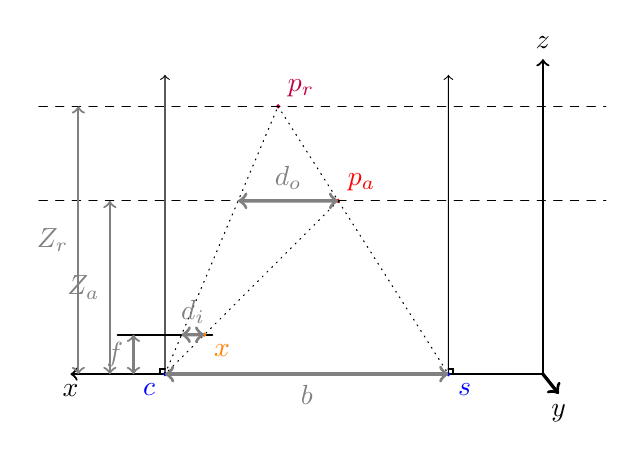
\begin{tikzpicture}[scale=0.40,cap=round]

    % let's define some key values
    \def\xc{-12}
    \def\xs{-3}
    \def\yimageplanes{1.25}
    \def\imageplaneshalfwidth{1.5}
    \def\xdistoffsetf{\imageplaneshalfwidth  + 0.5}
    \def\xdistoffsetZa{\imageplaneshalfwidth  - 0.25}
    \def\xdistoffsetZr{\imageplaneshalfwidth  - 1.25}
    \def\ydistoffsetxl{\yimageplanes + 0.125}
    \def\ydistoffsetxr{\ydistoffsetxl}
    \def\ydistoffsetb{0}
    \def\ydistoffsetinterx{\ydistoffsetb}
    \def\xobject{-6.5}
    \def\objectdepth{5.5}
    \def\referencedepth{3 + \objectdepth}
    \coordinate (pa) at (\xobject,\objectdepth);
    \coordinate (s) at (\xs,0);
    \coordinate (c) at (\xc,0);
    \coordinate (rayl2) at (\xc,0);
    \coordinate (ipll) at (\xc - \imageplaneshalfwidth, \yimageplanes);
    \coordinate (iplr) at (\xc + \imageplaneshalfwidth, \yimageplanes);


    % intersections of normals and reference plane
    \coordinate (rnrdi) at (\xs, \referencedepth);
    \coordinate (lnrdi) at (\xc, \referencedepth);
    % intersections of normals and object plane
    \coordinate (rnodi) at (\xs, \objectdepth);
    \coordinate (lnodi) at (\xc, \objectdepth);

    \coordinate (pr) at (intersection of s--pa and lnrdi--rnrdi);

    % intersection of c -- pr and object plane
    \coordinate (cprodi) at (intersection of c--pr and rnodi--lnodi);

    % pixel on image plane and expected pixel on image plane
    \coordinate (pixel) at (intersection of ipll--iplr and pa--c);
    \coordinate (epixel) at (intersection of ipll--iplr and pr--c);

    % Styles
    \tikzstyle{axes}=[]

    \begin{scope}[style=axes]
    \draw[->, thick] (0,0) -- (-15,0) node (xaxis) [below] {$x$};
    \draw[->, thick] (0,0) -- (0,10) node (zaxis) [above] {$z$};
    \draw[->, very thick] (0,0) -- (0.5,-0.625) node [below] {$y$};

    \end{scope}

    % point on object
    \draw [fill, red] (pa) circle (0.05) node [above right] {$p_a$};

    % point on reference plane
    \draw [fill, purple] (pr) circle (0.05) node [above right] {$p_r$};

    % left camera
    \draw [fill, blue] (-12,0) circle (0.05) node [below left] {$c$};
    % left image plane
    \draw[-, thick] (\xc - \imageplaneshalfwidth,\yimageplanes) -- 
        (\xc + \imageplaneshalfwidth, \yimageplanes);

    % right camera
    \draw [fill, blue] (-3,0) circle (0.05) node [below right] {$s$};

    % depth plane
    \draw[dashed, domain=-16:2] plot (\x, {\objectdepth});
     
    % Reference plane
    \draw[dashed, domain=-16:2] plot (\x, {\referencedepth});
    % p_r

    % image ray
    \draw[dotted] (pa)--(c);

    % projection ray
    \draw[dotted] (pr)--(s);
    
    % expected image ray
    \draw[dotted] (c)--(pr);

    % image points
    \draw[fill, orange] (pixel) circle (0.05) node [below right] {$x$};

    % focal length
    \draw[<->, thick, gray] (\xc - \xdistoffsetf,0) -- (\xc - \xdistoffsetf,\yimageplanes)
        node [midway, left, gray] {$f$};
    
    % Camera norms
    % left
    \draw[->] (c) -- (\xc, \referencedepth + 1);
    % perpendicular symbol
    \draw[thick] (\xc,0.15) -| (\xc-0.15, 0); 
    % right
    \draw[->] (s) -- (\xs, \referencedepth + 1);
    % perpendicular symbol
    \draw[thick] (\xs,0.15) -| (\xs +0.15, 0); 
    %(\xs,0)
    
    % actual depth
    \draw[<->, thick, gray] (\xc - \xdistoffsetZa, 0)
        -- (\xc - \xdistoffsetZa, \objectdepth)
        node [midway, left, gray] {$Z_{a}$};
    % reference depth
    \draw[<->, thick, gray] (\xc - \xdistoffsetZr, 0)
        -- (\xc - \xdistoffsetZr, \referencedepth)
        node [midway, left, gray] {$Z_{r}$};
    
    % camera distance
    \draw[<->, very thick, gray] (\xc,\ydistoffsetb) -- (\xs,\ydistoffsetb)
        node [midway, below, gray] {$b$};
    
    % point disparity over epipolar line
    \draw[<->, very thick, gray] (cprodi) -- (pa) node [midway, above, gray] {$d_o$};
    % point disparity over image plane
    \draw[<->, very thick, gray] (epixel) -- (pixel) node [midway, above, gray] {$d_i$};
    
\end{tikzpicture}
